\section{実装}
本章では提案システムの実装について述べる。まず3章で述べた設計を実装する際に生じる課題の解決方法について述べた後、システムの動作について述べる。

%現在の提案システムの実装はサーバマシンとクライアントマシンがXMPPサーバから取得した情報をもとに直接リンクを張ってクラウドゲーミング通信を展開する方式になっている。クラウドゲームサーバ/クライアントにはオープンソースクラウドゲーミングプラットフォームであるGamingAnywhereを使用している。また、パブリッククラウド等で展開しているサービスではなく、一般のユーザコンピュータでサービスを展開する手法特有の課題とその対処についても本章で述べる。


%以下ではそれぞれの課題の解決方法を述べる。

\subsection{VCコントローラとエージェントの連携}
VCコントローラと遊休コンピュータ上で動作するVCホストエージェントとの通信の課題についてはgRPC\cite{grpc}を用いる。gRPCはGoogleが開発しているオープンソースのRPCフレームワークで、異なるコンピュータ間情報をやり取りするために使用される。gRPCではクライアントアプリケーションがローカルで実装されたメソッドを使用するかのようにサーバアプリケーションのメソッドを直接呼び出すことができるため、分散アプリケーション等の実装に適している(図\ref{fig:grpc})。サーバ側ではサービスを定義してそのインターフェースを実装する。クライアント側ではサーバと同じメソッドを提供するスタブを介してサーバアプリケーションの機能を使えるようにしているのが特徴である。

gRPCのResponse Streaming gRPCという機能は、単一の要求に対して複数のレスポンスを任意のタイミングで返すことが可能である。これを使用することで、VCクライアントが送信した単一のゲームプレイ要求に対して、ACKや起動報告、実行終了時の完了報告、エラーの通知など様々なレスポンスを返すことができる。

\begin{figure*}[t]
    \centering
    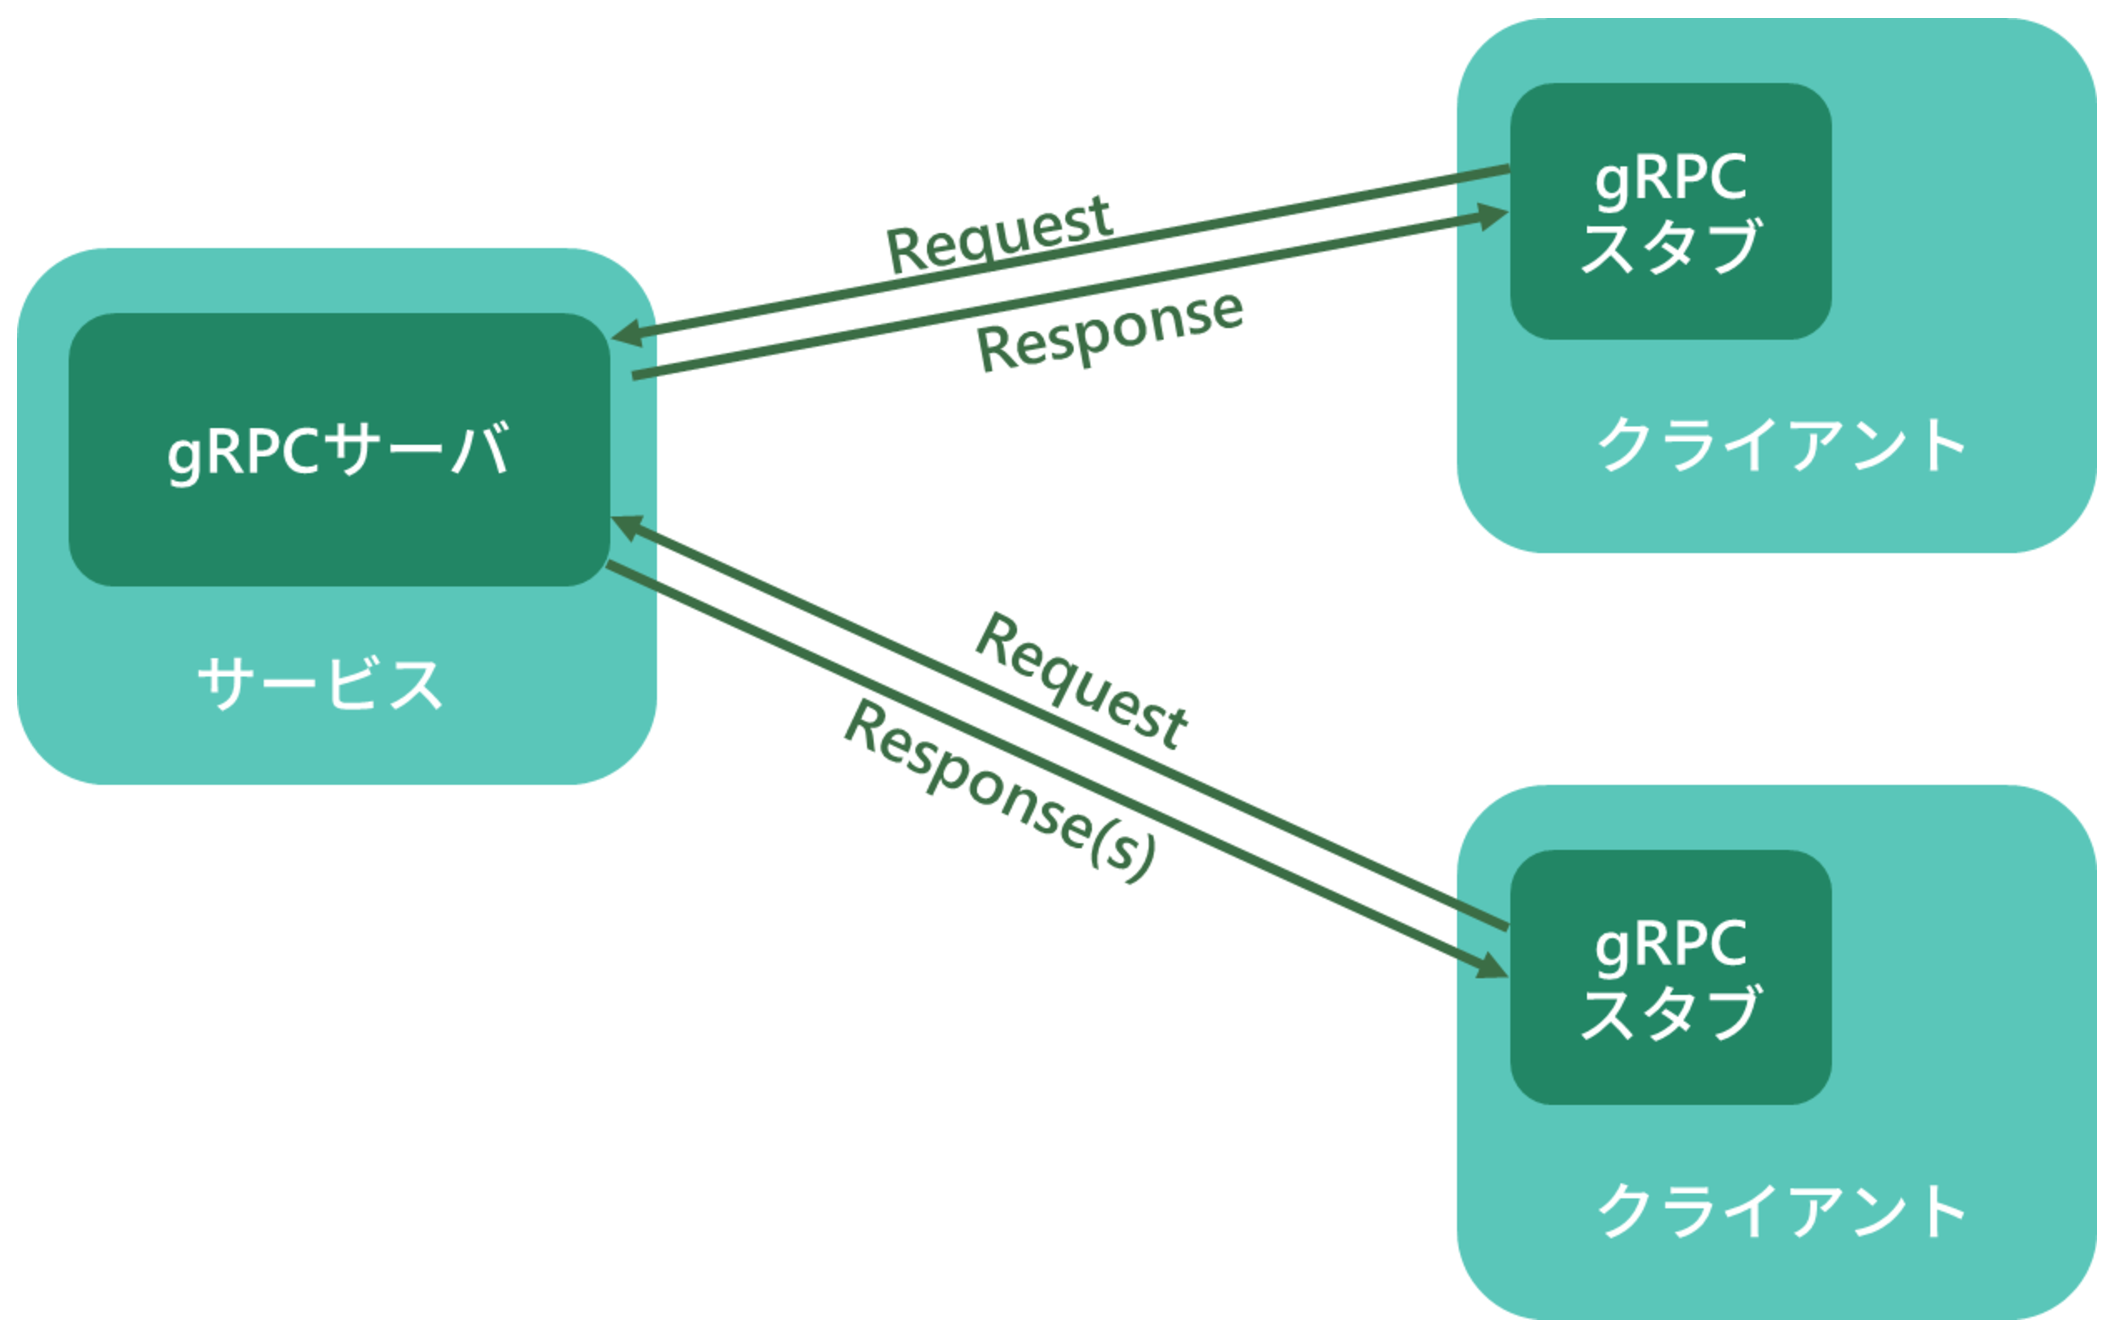
\includegraphics[width=0.8\textwidth,keepaspectratio,clip]{img/grpc.eps}
    \caption{gRPCの概要}
    \label{fig:grpc}
\end{figure*}

\subsection{クラウドゲームサーバ/クライアント間のP2P通信}
実際にリモートでのゲームプレイを実現するクラウドゲームサーバとクラウドゲームクライアントにはGamingAnywhereを使用する。GamingAnywhereはオープンソースのクラウドゲーミングプラットフォームであり、ユーザのコンピュータにインストールして設定を最適に変更しつつ実験を行えるクラウドゲームテストベッドである。遊休コンピュータ上にGamingAnywhereサーバ、プレイヤーPC上にGamingAnywhereクライアントを起動し、GamingAnywhereサーバが展開するRTSPサーバにクライアントが接続することでクラウドゲームのプレイが開始される。

ここで、ユーザコンピュータで動作するGamingAnywhereサーバ/クライアント間で双方向的な直接通信を行えないという問題がある。これを解決するため、GamingAnywhereの通信を行うリンクに対しEdgeVPN\cite{edgevpn}を使用する。EdgeVPNは、分散エッジソース全体にスケーラブルVPNを展開するためのオープンソースソフトウェアである。パケットキャプチャ、暗号化、トンネリング、転送およびNATトラバーサルのサポートが組み込まれている。エッジデバイスとNAT/ファイアウォール、およびクラウドコンピューティングリソースの背後にあるネットワークアドレスに透過的に接続することで、インターネットを介したトラフィックをP2Pで暗号化およびトンネリングすることができる。EdgeVPNリンクはオープンソースのWebRTCフレームワークによって実装されたSSLベースのトランスポートレイヤプロトコルセキュリティで暗号化および認証され、ノード間の通信はトンネルを介してUDPに基づくDatagram TLS(DTLS)\cite{dtlc}を使用する。また、EdgeVPNはXMPPプロトコル\cite{xmpp}を使用してピアとの接続情報を検出および交換する。パケット交換とルーティングは分散されているため、スケーラブルなP2Pオーバレイを展開しつつ、メンバーシップの一元管理も可能である。

EdgeVPNはSt Justeら\cite{tincan}が開発したTinCanに基づいている。TinCanは、XMPPサーバを使用してエンドツーエンドのVPNトンネルをブートストラップし、分離されたコントローラ/データパスモデルをサポートしている。また、ノードが接続先にパブリックIPやポートを知らせるためのリフレクションサービスとしてSTUNプロトコル\cite{stun}を使用し、制限の強いファイアウォールやSymmetric NATの背後にあり直接P2P接続を構築できないノードがある場合はリレーサービスとしてTURNプロトコル\cite{turn}を使用してトラフィックをプロキシしている。

\subsection{システム動作}
本節ではシステムの動作のシーケンスについて述べる。まず始めにクラウド上に存在するXMPPサーバを使用して、プレイヤーPCと遊休コンピュータがgRPCおよびEdgeVPNのリンクを張るための接続情報をそれぞれに通知する(図\ref{fig:seq}矢印1)。次に、プレイヤーの希望に応じて、プレイヤーPC上のVCクライアントエージェントがgRPCクライアントとして、遊休コンピュータで動作するVCホストエージェント上のgRPCサーバにゲーム起動要求を送信する(矢印2)。これを受信したVCホストエージェントは、クラウドゲームサーバの役割を果たすGamingAnywhereサーバとプレイヤーが指定した所望のゲームを起動し(矢印3)、GamingAnywhereサーバがゲーム画面のキャプチャを開始した後(矢印4)、了解を返す(矢印5)。その後、遊休コンピュータとプレイヤーPC間にEdgeVPNのリンクを張り、プレイヤーPCがGamingAnywhereクライアントを起動して、トンネルを介してGamingAnywhereサーバに接続することでゲームプレイを開始する(矢印6)。また、ゲームプレイ終了時はGamingAnywhereクライアントの終了によって接続の切断がGamingAnywhereサーバに通知されるため、それを観測することでVCクライアントエージェントは終了を検知し、GamingAnywhereとゲームを終了する(矢印7)。

\begin{figure*}[t]
    \centering
    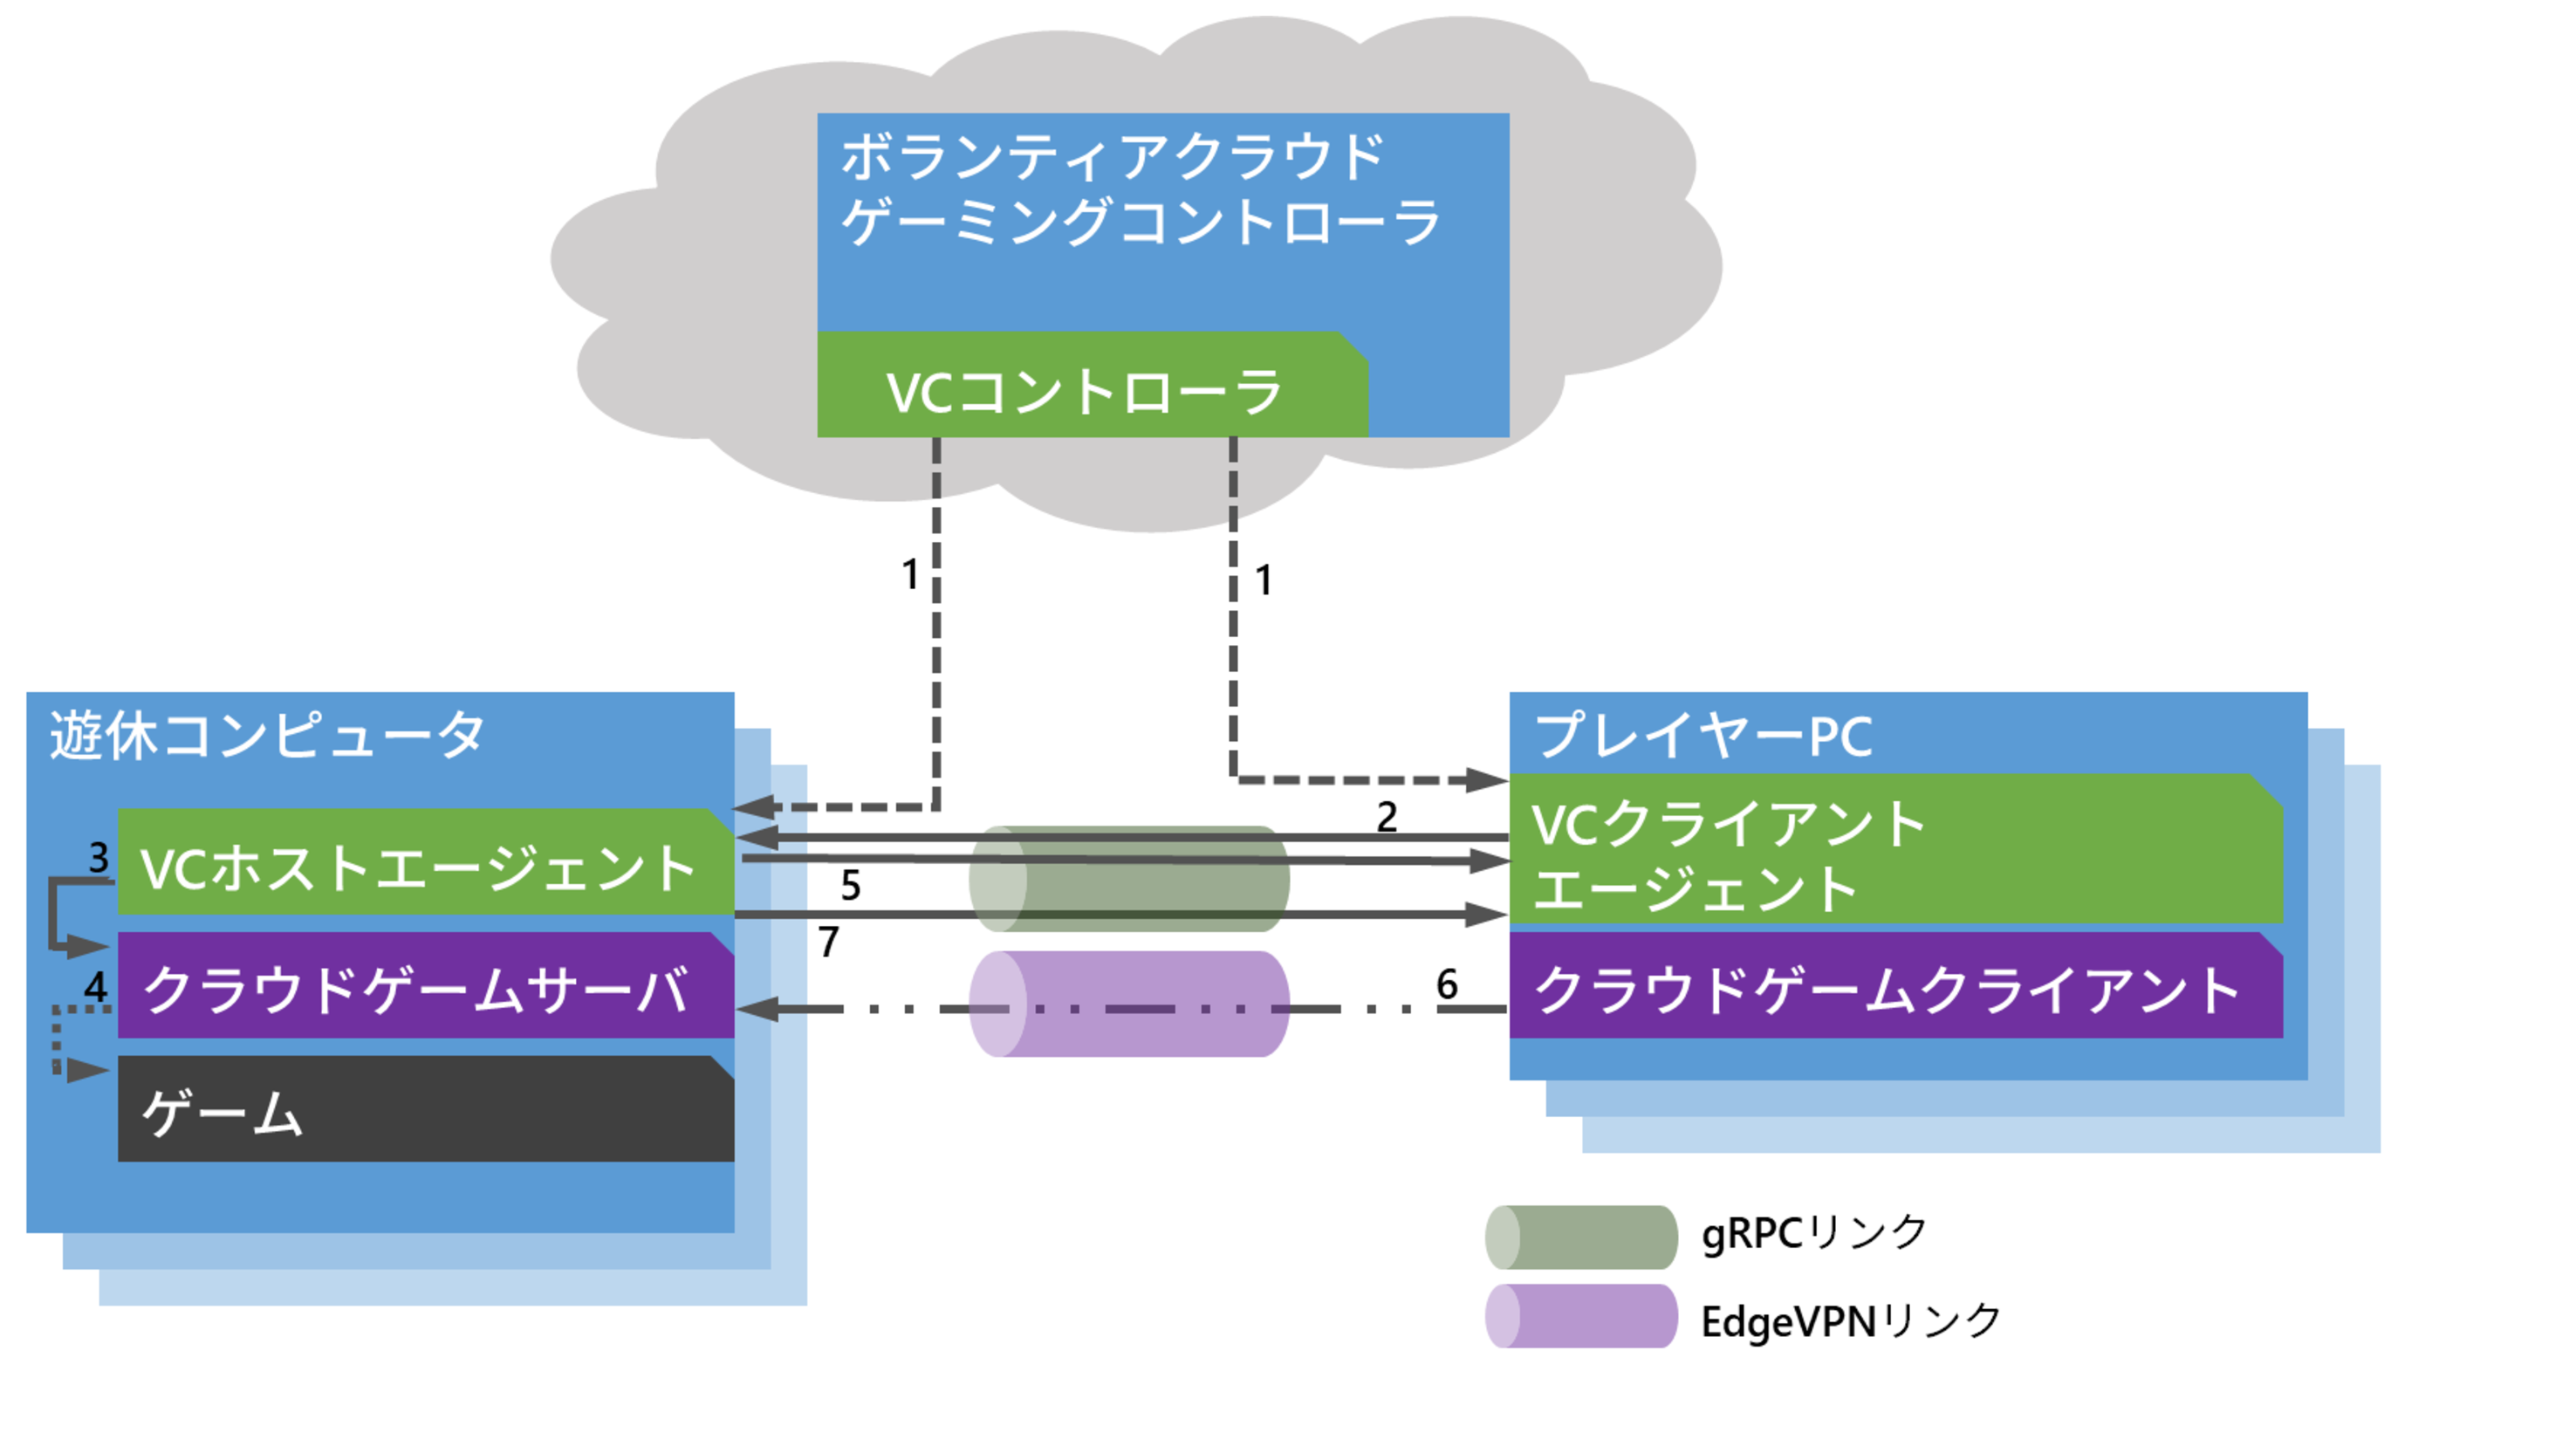
\includegraphics[width=0.8\textwidth,keepaspectratio,clip]{img/sequence.eps}
    \caption{システム動作}
    \label{fig:seq}
\end{figure*}

